\documentclass[10pt]{article}
\usepackage[utf8]{inputenc}
\usepackage[italian]{babel}
\usepackage{multicol}
\usepackage{amssymb}
\usepackage{amsfonts}
\usepackage[bookmarks]{hyperref}
\usepackage[a4paper, total={18cm, 25cm}]{geometry}
\usepackage{graphicx}
\usepackage{xcolor}
\usepackage{textcomp}
\graphicspath{ {.} }
\usepackage{listings}
\usepackage{makecell}
\usepackage{qtree}
\usepackage{pgfplots}
\usepackage{tikz}
\usetikzlibrary{quantikz, shapes, arrows}
\usepackage{blochsphere}
\usepgflibrary{shapes}
\usepackage{cancel}
\usepgfplotslibrary{fillbetween}
\definecolor{backcolour}{RGB}{255,255,255}
\definecolor{codegreen}{RGB}{27,168,11}
\definecolor{codeblue}{RGB}{35,35,205}
\definecolor{codegray}{RGB}{128,128,128}
\definecolor{codepurple}{RGB}{205,35,56}
\lstdefinestyle{myPython}{
	backgroundcolor=\color{backcolour},   
	commentstyle=\color{codegreen},
	keywordstyle=\color{codeblue},
	numberstyle=\tiny\color{codegray},
	stringstyle=\color{codepurple},
	basicstyle=\small\ttfamily,
	breakatwhitespace=false,         
	breaklines=true,                 
	captionpos=b,                    
	keepspaces=true,                 
	numbers=left,                    
	numbersep=2pt,                  
	showspaces=false,                
	showstringspaces=false,
	showtabs=false,                  
	tabsize=2,
	language=python
}
\newcommand*\triangled[1]{\tikz[baseline=(char.base)]{
            \node[regular polygon, regular polygon sides=3,draw,inner sep=1pt] (char) {#1};}}
            
\usepackage{fancyhdr}
\pagestyle{fancy}
\renewcommand{\headrulewidth}{0pt}
\fancyhead{}
\begin{document}
\title{Parallel Implementation of Huffman Coding}
\author{Federico Matteoni}
\date{A.A. 2022/23}
\maketitle

%The report submitted along with the project code:
%• Should be at most 10 pages
%• Should not include known material, such as project problem description, known performance formulas, and so on
\section{The Alternatives}
Huffman coding may be implemented in different ways. Huffman uses a table containing the number of occurrences of each symbol in the input text. The goal is to assign a unique sequence of bits to each symbol in an optimal way, meaning that the encoding of each character must have a unique prefix to unambiguously differentiate each character. This is achieved by arranging the characters in a binary tree: by assigning each subtree a 0/1 value, the code for each character is found by traversing the tree from the root to the leaf, concatenating the found 0/1s.\\
Building such tree is the key of the Huffman Coding algorithm.
\paragraph{Greedy} The first approach that comes to mind can be defined as a greedy approach. Given our $n$ characters, the idea is to start with a tree rooted in a fake node with $n$ subtrees, each representing one of the characters. Then, iteratively, we combine two nodes with the smallest weights into a tree, assigning as weight the sum of the two original nodes. This loops until we end up with a binary tree.\\
This approach involves sorting the characters based on the frequencies, requiring $O(n\cdot\log n)$ for $n$ characters, $O(n-1)$ steps of merging pairs of nodes and updating the overall tree. This results in a $O(n\cdot\log n)$ complexity.
\paragraph{Top-Down} Another approach is to build the tree in a top-down fashion. We consider all possible ways of dividing the characters in the two subtrees, and once the decision is taken we recursively do the same for both subtrees.\\
This algorithm involves a binary decision for each of the characters, thus resulting in an exponential ($O(2^n)$ for $n$ characters) algorithm.
\paragraph{Heap} The chosen implementation involves using an heap to store and encode the Huffman tree. This way, using a well-known and understood data structure, we may exploit different kinds of optimizations. The time complexity of traversing the heap, action involved in determining the smallest weights and inserting the nodes, is $O(n\cdot\log n)$. The advantage is that we maintain a single tree, and won't perform additional actions that will add overhead like in the greedy approach.
\section{Implementation}
The implementation phase of the project begins with the sequential program. The sequential approach has been used to implement and test all the basic functionality of the heap, with data structures, node insertion logic, codes generation and file reading/writing utilities. The sequential approach was useful in determining bugs in the heap implementation, validating the generated encoding and checking the memory usage of the overall project.
\paragraph{Data} The remote machine has been built with particularly powerful components. This means that even slow and not efficient implementation could prove to be very fast on small files, not yielding significative time differences between the three implementations.\\
The testing data involves the "Lorem Ipsum Dolor" paragraphs, with few variations to test different aspects of the implementation early on (e.g. handling uppercase-lowercase letters, symbols and so on). The final testing file, called \texttt{longfile}, has been crafted by copy-pasting few paragraphs until the sequential approach took few seconds to complete its computing when compiled without optimizations (without the \texttt{-O3} flag). This provided a fairly good benchmark to start with, and lets the user appreciate the difference between optimized and non optimized binaries, as well as the difference between sequential and parallel code.
\paragraph{Memory Usage} One particular obstacle that could be faced during the implementation of all three approaches (sequential, thread-based and fastflow-based) was memory usage. In particular, an initial approach used variables and arrays declared in classic C++99 style, thus requiring an heavy usage of \texttt{malloc}s and \texttt{free}s. This approach is error-prone given the logic of the heap that needs to be implemented and the flow of data between the modules. The solution was and early migration to more modern data structures, like \texttt{std::vector}s and \texttt{shared\_ptr}s/\texttt{unique\_ptr}s. By exploiting their constructors and destructors, memory management was solved. The only memory that's left to be explicitly managed are fastflow's pointers.
\paragraph{Code Reuse} An aspect of the presented implementations is the heavy relying on code reuse. One of the key aspects on parallel programming is the ability to reuse sequential code whenever possible, with the goal of exploiting optimizations and ideas that were implemented throughout the years of studying a certain problem. While this is certainly not the case for this particular project, as all the code has been written from scratch, to emulate this kind of approach all the code that is not directly involved in the flow of computation, whether it being sequential or parallel, has been placed in a small library (the file \texttt{huffman.cpp}) and reused as much as possible.\\
This goal has certainly proved to be a particularly difficult approach, but also a time-saving one. By implementing, and testing, only one logic responsible for reading/writing files, building the heap, generating the codes given the final heap, and so on, the only "new code" that were needed was an efficient orchestration of the parallel computation that used the already written-and-tested sequential code.
\section{Evaluation}
%• Should include experiments performed on the remote virtual machine, with proper plots (B&W only, please do not use colors)
\begin{center}
	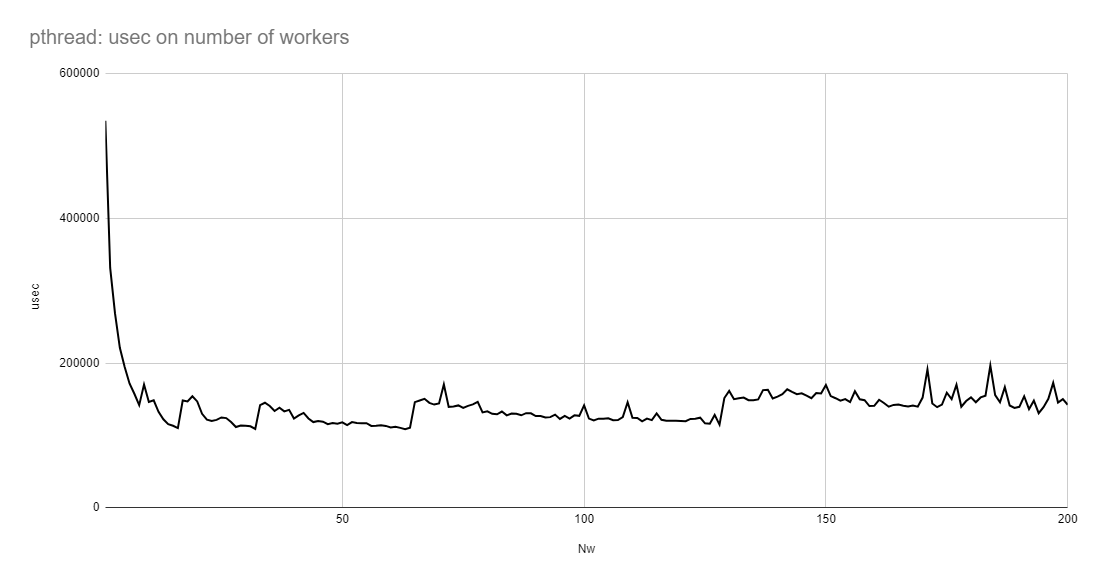
\includegraphics[scale=.5]{scalability_pthreads.png}\\
	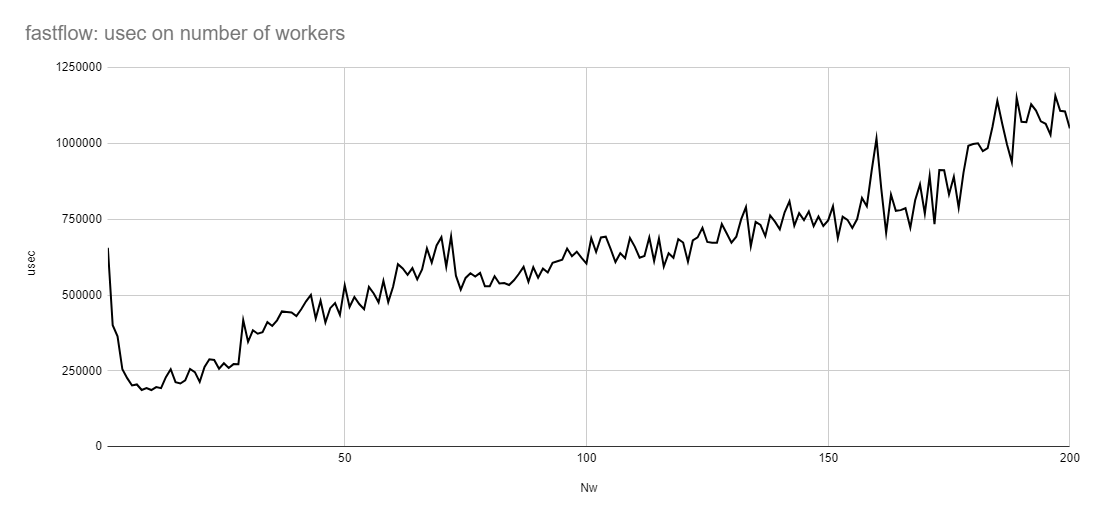
\includegraphics[scale=.5]{scalability_fastflow.png}
\end{center}
\section{Discussion}
%• Should include some discussion relative to the motivation of the differences between achieved performance figures and the ideal/predicted ones, in particular pointing out qualitatively and quantitively, the major sources of overhead.
\section{Running the Code} 
%• Should include the instructions needed to compile and run the code
\end{document}  
